\chapter{Can Quantum-Mechanical Description of Reality Be Considered Complete?\label{EPR}}
\chapterprecis{Einstein, Podolsky, and Rosen\footnote{\emph{Physical Review} \textbf{47} (1935),
  777--80. }}

% Original citation had: ``Reprinted in \emph{QTM} 138--41.'' What is QTM?

\makeoddhead{myheadings}{\emph{Einstein, Podolsky, and Rosen}}{}{\thepage}
\makeevenhead{myheadings}{\thepage}{}{\emph{Can Quantum-Mechanical Description of 
Reality Be Considered Complete?}}

\renewcommand{\theequation}{\arabic{equation}}

\subsection*{1.}

Any serious consideration of a physical theory must take into account
the distinction between the objective reality, which is independent of
any theory, and the physical concepts with which the theory operates.
These concepts are intended to correspond with the objective reality,
and by means of these concepts we picture this reality to ourselves.

In attempting to judge the success of a physical theory, we may ask
ourselves two questions: (1) ``Is the theory correct?'' and (2) ``Is the
description given by the theory complete?'' It is only in the case in
which positive answers may be given to both of these questions, that the
concepts of the theory may be said to be satisfactory. The correctness
of the theory is judged by the degree of agreement between the
conclusions of the theory and human experience. This experience, which
alone enables us to make inferences about reality, in physics takes the
form of experiment and measurement. It is the second question that we
wish to consider here, as applied to quantum mechanics.

Whatever the meaning assigned to the term \emph{complete,} the following
requirement for a complete theory seems to be a necessary one:
\emph{every} \emph{element of the physical reality must have a
counterpart in the physical theory.} We shall call this the condition of
completeness. The second question is thus easily answered, as soon as we
are able to decide what are the elements of the physical reality.

The elements of the physical reality cannot be determined by a priori
philosophical considerations, but must be found by an appeal to results
of experiments and measurements. A comprehensive definition of reality
is, however, unnecessary for our purpose. We shall be satisfied with the
following criterion, which we regard as reasonable. \emph{If, without in
any way disturbing a system, we can predict with certainty (i.e.,}
\emph{with probability equal to unity) the value of a physical}
\emph{quantity, then there exists an element of physical} \emph{reality
corresponding to this physical quantity.} It seems to us that this
criterion, while far from exhausting all possible ways of recognizing a
physical reality, at least provides us with one such way, whenever the
conditions set down in it occur. Regarded not as a necessary, but merely
as a sufficient, condition of reality, this criterion is in agreement
with classical as well as quantum-mechanical ideas of reality.

To illustrate the ideas involved let us consider the quantum-mechanical
description of the behavior of a particle having a single degree of
freedom. The fundamental concept of the theory is the concept of
\emph{state}, which is supposed to be completely characterized by the
wave function $\psi$, which is a function of the variables chosen to
describe the particle's behavior.\\
\centerline{* * *}
%
A definite value of the [spatial] coordinate, for a particle in [the sort of state
described by quantum mechanics] is thus not predictable, but may be obtained
only by a direct measurement. Such a measurement however disturbs the
particle and thus alters its state. After the coordinate is determined,
the particle will no longer be in the {[}same{]} state\ldots. The usual
conclusion from this in quantum mechanics is that \emph{when the
momentum of a particle is known, its coordinate has no physical
reality}.

More generally, it is shown in quantum mechanics that, if {[}two
physical quantities are in the indeterminacy relation to each other,{]}
then the precise knowledge of one of them precludes such a knowledge of
the other. Furthermore, any attempt to determine the latter
experimentally will alter the state of the system in such a way as to
destroy the knowledge of the first.

From this follows that either (1) \emph{the quantum-mechanical
description of reality given by the wave function is not complete} or
(2) \emph{when {[}two physical quantities are in the indeterminacy
relation to each other,{]} the two quantities cannot have simultaneous
reality}. For if both of them had simultaneous reality---and thus
definite values---these values would enter into the complete
description, according to the condition of completeness. If then the
wave function provided such a complete description of reality, it would
contain these values; these would then be predictable. This not being
the case, we are left with the alternatives stated.

In quantum mechanics it is usually assumed that the wave function
\emph{does} contain a complete description of the physical reality of
the system in the state to which it corresponds. At first sight this
assumption is entirely reasonable, for the information obtainable from a
wave function seems to correspond exactly to what can be measured
without altering the state of the system. We shall show, however, that
this assumption, together with the criterion of reality given above,
leads to a contradiction.

\subsection*{2.}

For this purpose let us suppose that we have two systems, I and II,
which we permit to interact from the time \emph{t} = 0 to \emph{t} =
\emph{T}, after which time we suppose that there is no longer any
interaction between the two parts. We suppose further that the states of
the two systems before \emph{t} = 0 are known.

[Because of the mathematics involved, we will not be able to follow the
example constructed by Einstein, Podolsky, and Rosen. However Bohr has
described\footnote{In his reply to the EPR paper, itself entitled ``Can quantum-mechanical 
description of physical reality be considered complete?'' \emph{Physical Review} 
\textbf{48} (1935), 696–-702.} a thought-experiment which, he claims,
captures the essential features of the EPR argument:]

\begin{quote}
The particular quantum-mechanical state of two free particles, for which
they {[}i.e., EPR{]} give an explicit mathematical expression, may be
reproduced, at least in principle,\footnote{The obvious impossibility of
  actually carrying out, with the experimental technique at our
  disposal, such measuring procedures as are discussed here and in the
  following does clearly not affect the theoretical argument, since the
  procedures in question are essentially equivalent with atomic
  processes, like the Compton effect, where a corresponding application
  of the conservation theorem of momentum is well established.} by a
simple experimental arrangement, comprising a rigid diaphragm with two
parallel slits, which are very narrow compared with their separation,
and through each of which one particle with given initial momentum
passes independently of the other. If the momentum of this diaphragm is
measured accurately before as well as after the passing of the
particles, we shall in fact know the sum of the components perpendicular
to the slits of the momenta of the two escaping particles, as well as
the difference of their initial positional coordinates in the same
direction;\footnote{{[}Let $p_1$ and $p_2$ be the vertical
  components of the momentum of the particles after they have passed
  through the top and bottom slits, respectively. And let $P$ be
  the vertical component of the momentum of the diaphragm after the two
  particles have passed through the slits. If we assume that before the
  particles pass through the slits the vertical components of the
  momentum of the two particles and of the diaphragm were all zero, then
  by the conservation of momentum, $p_1 + p_2 = -P$.\\
  Let $x_1$ and $x_2$ be the coordinates of the vertical
  position of the particles just after they have passed through the top
  and bottom slits, respectively. And let $d$ be the distance
  between the two slits. Then just after the two particles pass through
  the slits, $x_1 - x_2 = d$.]\label{entangle}} while of course the
\ldots{} difference of the components of their momenta, and the sum of
their positional coordinates, are entirely unknown. In this arrangement,
it is therefore clear that a subsequent single measurement either of the
position or of the momentum of one of the particles {[}namely, system
I{]} will automatically determine the position or momentum,
respectively, of the other particle {[}system II{]} with any desired
accuracy; at least if the wave-length corresponding to the free motion
of each particle is sufficiently short compared with the width of the
slits.\footnote{{[}In his account of his discussions with Einstein, Bohr
  includes the figure below on the left to illustrate a similar
  experiment involving only one slit. Below on the right is a figure
  illustrating the double-slit experiment; the detector is a Geiger
  counter.{]}
\begin{center}
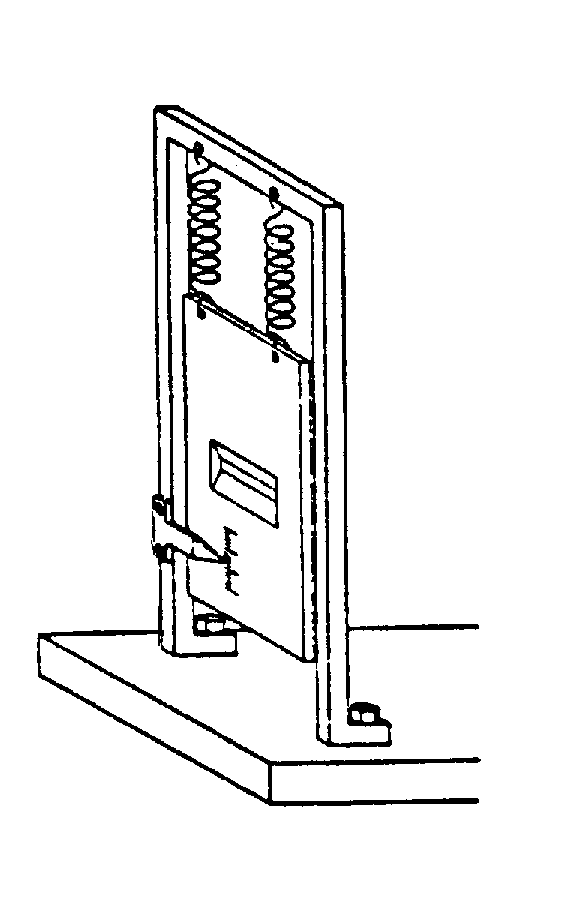
\includegraphics[width=0.76944in,height=1.19236in]{images/16_epr/image017.png}
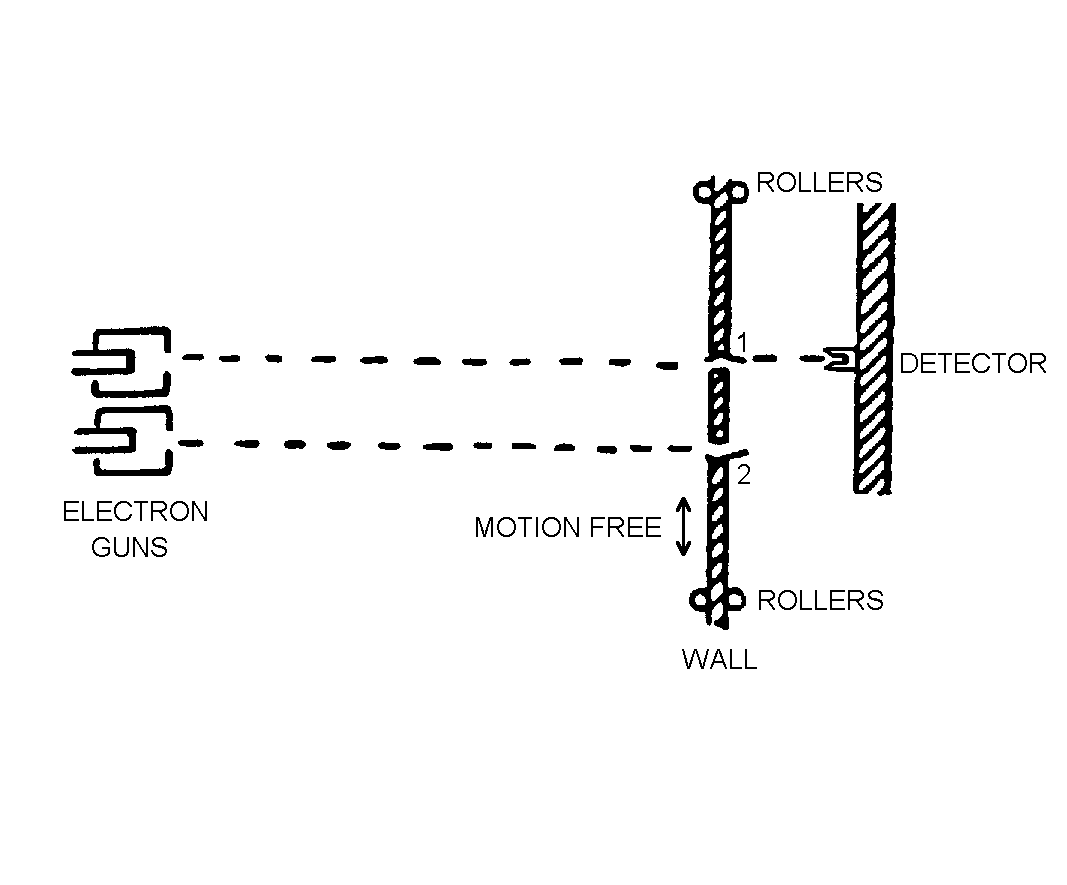
\includegraphics[width=1.77833in,height=1.475in]{images/16_epr/image019.png}
\end{center}
}
\end{quote}

[EPR continue:]

We see therefore that, as a consequence of two different measurements
performed upon the first system, {[}either the position or the momentum
of the second system may be measured with any desired accuracy{]}. On
the other hand, since at the time of measurement the two systems no
longer interact, no real change can take place in the second system in
consequence of anything that may be done to the first system. This is,
of course, merely a statement of what is meant by the absence of an
interaction between the two systems.\\
\centerline{* * *}
%
Thus, by measuring either {[}the position of I{]} or {[}the momentum of
I,{]} we are in a position to predict with certainty, and without in any
way disturbing the second system, either the value of the {[}position{]}
or the value of the {[}momentum of the second system{]}. In accordance
with our criterion of reality, in the first case we must consider the
{[}position of II{]} as being an element of reality, in the second case
the {[}momentum of II{]} is an element of reality\ldots.

Previously we proved that either (1) the quantum-mechanical description
of reality given by the wave function is not complete or (2) \emph{when
{[}two physical quantities are in the indeterminacy relation to each
other,{]} the two quantities cannot have simultaneous reality}. Starting
then with the assumption that {[}quantum mechanics{]} does give a
complete description of the physical reality, we arrived at the
conclusion that two physical quantities, {[}which are related by the
indeterminacy relations{]}, can have simultaneous reality. Thus the
negation of (1) leads to the negation of the only other alternative (2).
We are thus forced to conclude that the quantum-mechanical description
of physical reality given by wave functions is not complete.

One could object to this conclusion on the grounds that our criterion of
reality is not sufficiently restrictive. Indeed, one would not arrive at
our conclusion if one insisted that two or more physical quantities can
be regarded as simultaneous elements of reality \emph{only when they can
be} \emph{simultaneously measured or predicted.} On this point of view,
since either one or the other, but not both simultaneously, of the
quantities {[}momentum{]} and {[}position of the second system{]} can be
predicted, they are not simultaneously real. This makes the reality of
{[}the momentum{]} and {[}position of the second system{]} depend upon
the process of measurement carried out on the first system, which does
not disturb the second system in any way. No reasonable definition of
reality could be expected to permit this.

While we have thus shown that the wave function does not provide a
complete description of the physical reality, we left open the question
of whether or not such a description exists. We believe, however, that
such a theory is possible.\\
\centerline{* * *}
%